\documentclass[a4paper]{article}
\usepackage{graphicx} % Required for inserting images
\usepackage{indentfirst}
\usepackage[brazil]{babel}
\usepackage{amssymb}
\usepackage{amsmath}
\usepackage{dsfont}
\usepackage[left=2.5cm,top=2.5cm,right=2.5cm,bottom=2.5cm]{geometry}
\usepackage{tikz}
\usepackage{float}
\graphicspath{ {./images/} }

\title{Estimativa de integrais utilizando Métodos Monte Carlo - MAP2212}
\author{Antonio Gabriel Freitas da Silva - 13687290}
\date{Maio 2023}

\begin{document}

\maketitle

\section{Introdução}

Os métodos de integração de Monte Carlo servem para tentar estimar a área de uma função de forma mais eficiente em aspectos computacionais. Este trabalho tem como objetivo principal a demonstração dos quatros principais métodos integração Monte Carlo, assim como a suas vantagens e desvantegens e uma simulação de uma função dada como $f(x) = \exp{(-0.32798830x)}\cdot\cos{(0.04715069237x)}$ no intervalo $[0,1]$.

\section{Sobre os métodos}

\subsection{Método Crude}
O método Crude ("bruto", no português) seria considerada a forma mais casual de se calcular uma integral por Monte Carlo, ao termos uma estimativa de uma média $\gamma$ dada por $\hat{\gamma_{c}}$, tal que:

\begin{center}

$\gamma = \int_{a}^{b} f(x) dx$, com $\sigma_{c}^{2} = \frac{1}{n}\int_{a}^{b} (f(x) - \gamma)^{2} dx$

\vspace{0.5cm}

$\hat{\gamma_{c}} = \frac{1}{n}\sum_{i = 1}^{n} f(x_{i}) $

\end{center}

A variância $\sigma_{c}^{2}$ será aproximada para o somatório $\frac{1}{n}\sum_{i = 1}^{n} (f(x_{i}) - \gamma)^{2}$. O cálculo dentro da função será realizado a partir de uma distribuição uniforme de parâmetros 0 e 1.

\subsection{Método Hit or Miss}

Considerado o método mais ineficiente para realizar estimativas, é realizada também uma distribuição de pontos dentro de um intervalo (que é dado como $[0,1]$) nos eixos x e y para o cada $f(x)$ nestas distribuições. O número de pontos dado como $n$ é dado a partir daqueles que estão dentro da função, a integral exata é dada por:

\begin{center}

$\gamma =  \iint_V f(x,y)dx\,dy$, que pode ser estimada por

\vspace{0.5cm}

$\hat{\gamma_{h}} = \frac{1}{n}\sum_{i = 1}^{n} f(x_{i}, y_{i}) $

\end{center}

A sua variância é baseada em uma distribuição Bernoulli, dada como $\sigma_{h}^2 = \hat{\gamma_{h}}(1-\hat{\gamma_{h}})$.

\subsection{Importance Sampling}

Este método tem uma diferença significativa em relação aos outros pelo fato de necessitar de uma distribuição de probabilidade $g(x)$ que se adeque mais para o estudo de uma função mais simples, de tal forma que o cálculo da área possua uma variância reduzida e uma média mais consistente. Sua forma de integração é dada por:

\begin{center}

$\gamma = \int_{a}^{b} \frac{f(x)}{g(x)}\cdot g(x) dx$, estimada como $\hat{\gamma_{i}} = \frac{1}{n}\sum_{i = 1}^{n} \frac{f(x_{i})}{g(x_i)} $

\vspace{0.5cm}

$\sigma_{i}^{2} = \frac{1}{n}\int_{a}^{b} (\frac{f(x)}{g(x)} - \gamma)^{2}g(x) dx$, estimada como $\hat{\sigma_{i}^{2}} = \frac{1}{n}\sum_{i=1}^{n} (\frac{f(x_i)}{g(x_i)}-\hat{\gamma_{i}})^2g(x_i)$

\end{center}

Podemos ver que cada distribuição se diferencia nos parâmetros que foram dados, temos a $\beta(1 , 1.1)$, $Weibull(0.6208, 1.4982)$ e $Gamma(1.0881, 3)$ ilustradas abaixo. Percebemos que a Beta é a melhor que se aproxima nesta ocasião, logo, esta será utilizada para o método de importance sampling.

\begin{figure}[H]
  \centering
  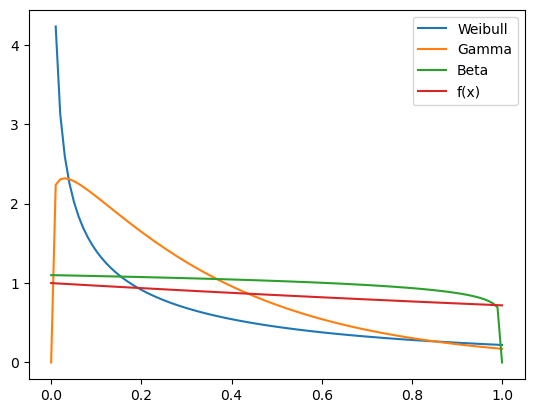
\includegraphics[width=0.7\textwidth]{Distribuições.png}
  \caption{f(x) comparadas a distribuições Beta, Gamma e Weibull}
  \label{fig:circulo}
\end{figure}


\subsection{Control Variates}

Sendo o melhor dos métodos para a estimação de um valor $n$ de amostras que melhor se encaixariam, podemos perceber que é viável utilizar um polinômio adequado para aproximarmos a função. Neste caso, utilizamos a função $\varphi(x) = -0.3x + 1$, que ao ser comparada, possui uma boa aproximação de $f(x)$ no intervalo $[0,1]$:

\begin{figure}[H]
  \centering
  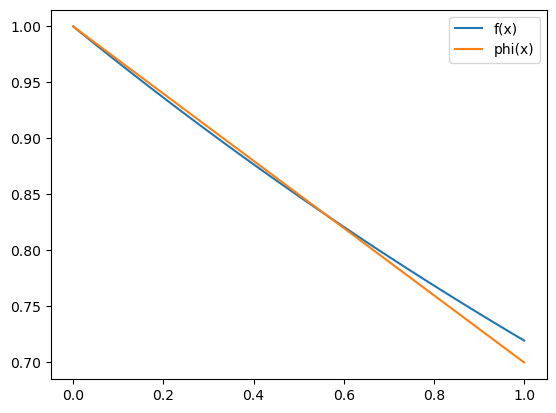
\includegraphics[width=0.7\textwidth]{Control.png}
  \caption{f(x) e $\varphi(x)$ para o método de Control Variates}
  \label{fig:Control}
\end{figure}

Assim, calculamos a área de $\varphi(x)$ como $\gamma' = \int_{0}^{1} -0.3x+1\,dx = 0.85$.
Ao termos ambas as funções, calculamos isto como:

\begin{center}

$\int_{a}^{b} (f(x) + \varphi(x) - \varphi(x)) \, dx$, estimada como $\hat{\gamma_v} = \frac{1}{n}\sum_{i = 1}^{n} (f(x_i) - \varphi(x_i) + \gamma')$ e sua variância dada por

\vspace{0.5cm}

$var(\hat{\gamma_v}) = var(f(x_i)) + var(\varphi(x_i)) - 2cov(f(x_i), \varphi(x_i))$

\end{center}

Calculamos os pontos de cada função a partir da distribuição uniforme de parâmetros 0 e 1.

\section{Cálculo do número de amostras}

Para isso, iremos utilizar os intervalos de confiança que serão mostrados a seguir:


\begin{center}

$\varepsilon = \frac{\sigma\cdot Z_{\alpha/2}}{\sqrt{n}} \implies n = (\frac{\sigma\cdot Z_{\alpha/2}}{\varepsilon})^2$

\end{center}

Utilizando como erro do tipo 1 do intervalo em $95\%$, logo, teremos um parâmetro $Z_{\alpha/2} = 1.96$ por regras de distribuição normal.

Queremos que o erro relativo esteja abaixo de $0.05\%$. Para os métodos Crude, Hit or Miss e Control Variates, consideramos que:

\begin{center}

$\frac{|\gamma - \hat{\gamma}|}{\hat{\gamma}} \le 0.0005 \implies \varepsilon = 0.0005\cdot \hat{\gamma}$

\end{center}

Agora, para o método de importance sampling, utilizamos como função secundária uma distribuição beta, de tal forma que não existe uma possibilidade de utilizar os parâmetros de uma distribuição normal para estimar um n novo, logo, para fins práticos, foi utilizado um método chamado "método da bissecção": temos dois limites inferior (número inicial de amostras) e superior (número inicial vezes 10), que enquanto não traz um erro relativo de $0.05\%$, divide os limites ao meio, calcula a nova integral e aumenta seu número de amostras até o valor desejado.

Pelo método de Hit or Miss ser o mais ineficiente em questão de tempo de execução de código, além de possuir a maior variância entre todas as outras variantes, temos que seu novo número amostral está na ordem de $10^6$ que, por si só, já garante precisão para aquelas outras, visto que precisam de valores menores para tal. No entanto, para fins de demonstração, temos abaixo um exemplo de simulação dos métodos utilizados.

\section{Exemplo de simulação e Conclusão}

\begin{table}[h]
\centering
\caption{Simulação com uma seed(9) e amostragem inicial n = 10000}
\vspace{0.5cm}
\begin{tabular}{r|lr}

Método & Integral estimada & Nova amostragem \\ % Note a separação de col. e a quebra de linhas
\hline                               % para uma linha horizontal
Crude & 0.852397       & 138222 \\
Hit or Miss & 0.851500   & 2679871 \\
Importance Sampling & 0.852259             & 55000  \\
Control Variates & 0.852282         & 921 \\

\end{tabular}
\end{table}

Dessa forma, podemos notar que o método mais eficiente para calcular um número de amostras menor, além de uma área mais precisa, é a Control Variates, no entando, ela demanda um tempo computacional maior que o Importance sampling, visto que será calculada uma maior quantidade de variâncias. O Hit or Miss, por ir na base de tentativa e erro, torna-se o pior dos métodos até para a sua estimação de amostragem nova. No entanto, cada método tem seu momento adequado de ser utilizado.

\end{document}
